\documentclass[12pt,aspectratio=169]{beamer}

\mode<presentation>
{
  \usetheme{Singapore}
  \setbeamersize{text margin left=.5cm,text margin right=.5cm}
%  \setbeamertemplate{navigation symbols}{} % suppress nav bar
%  \setbeamercovered{transparent}
}
\usefonttheme{professionalfonts}
\usepackage{graphicx}
\usepackage{tikz}
\usepackage{mathpazo}
\usepackage[scaled]{helvet}
\usepackage{xcolor,colortbl}
\usepackage{hyperref}
\usepackage{siunitx}


\sisetup{number-math-rm=\mathnormal}
%\sisetup{detect-all}


\title[Waves]{23.\ Mechanical Waves}
\subtitle{Advanced Placement Physics}
\author[TML]{Dr.\ Timothy Leung}
\institute{Olympiads School}
\date{Spring 2018}

\newcommand{\pic}[2]{\includegraphics[width=#1\textwidth]{#2}}
\newcommand{\eq}[2]{\vspace{#1}{\Large\begin{displaymath}#2\end{displaymath}}}


\begin{document}


\begin{frame}
  \titlepage
\end{frame}



\section{Waves}
\begin{frame}
  \frametitle{What is a wave?}
  \begin{itemize}
  \item When a disturbance (vibration) causes vibrations in its vicinity, a
    wave is created
  \item A wave transfers energy through a medium (there is one exception)
    \begin{itemize}
    \item The medium vibrates and have a net displacement of zero.
    \item Each particle vibrates instead of moving horizontally, and the
      vibration get transferred to the next particle.
    \end{itemize}
  \end{itemize}
\end{frame}



\begin{frame}
  \frametitle{Features of a Wave}
  \begin{itemize}
  \item\textbf{Crest}: Highest point
  \item\textbf{Trough}: Lowest point
  \item\textbf{Wavelength}: Shortest distance between two points in the medium
    that are in phase.
  \end{itemize}
  \begin{center}
    \vspace{-.5in}
    \pic{.8}{sine-wave1.png}
  \end{center}
  
  \vspace{-.3in}{\footnotesize(The easiest way to measure wavelength is from
    crest to crest, or from trough to trough.)\par}
\end{frame}



\begin{frame}
  \frametitle{Frequency and Speed of A Wave}

  Frequency of A Wave ($f$)
  \begin{itemize}
  \item The number of complete wavelengths that pass a point in a given amount
    of time
  \item Unit: hertz (\si{\hertz})
  \item Same as the frequency of the disturbance that generated the wave
  \item\textbf{Does not depend on the medium}, only the source that produces
    the wave.
  \end{itemize}

  \vspace{.2in}Speed of A Wave ($v$)
  \begin{itemize}
  \item The speed at which the wave fronts are moving
  \item\textbf{Depends only on the medium}
  \end{itemize}
\end{frame}


\begin{frame}
  \frametitle{Equation}
  A harmonic wave can be described as a sinusoidal function:
  \eq{-.1in}{
    \boxed{y(x,t)=A\sin(kx-\omega t)}
  }

  \begin{center}
    \begin{tabular}{l|c|l}
      \rowcolor{pink}
      \textbf{Quantity} & \textbf{Symbol} & \textbf{SI Unit} \\ \hline
      Displacement of the medium  & $y$ & \si{\metre} (meters)\\
      Wave number                 & $k$ & \si{/\metre} (per meter)\\
      Distance from the source    & $x$ & \si{\metre} (meters)\\
      Time                        & $t$ & \si{\second} (seconds)\\
      Angular frequency           & $\omega$ & \si{/\second} (per second)
    \end{tabular}
  \end{center}
\end{frame}


\begin{frame}
  \frametitle{Equation}
  \eq{-.1in}{
    \boxed{y(x,t)=A\sin(kx-\omega t)}
  }

  If the wave is generated by a mass on a spring, then $k$ is the spring
  constant of the spring. It is related to the wavelength by:
  
  \eq{-.2in}{
    k=\frac{2\pi}{\lambda}
  }

  \vspace{-.1in}The angular frequency (angular velocity) is related to the
  frequency $f$ and period $T$ of the wave by:

  \eq{-.35in}{
    \omega=\frac{2\pi}{T}=2\pi f
  }
\end{frame}


\begin{frame}
  \frametitle{Why Sine and Cosines}
  French mathematician Joseph Fourier discovered that \emph{all} periodic
  functions are infinite series of $\sin$ and/or $\cos$ functions:

  \vspace{-.35in}{\Large
    \begin{align*}
      f(x)=&a_1\sin(x)+a_2\sin(2x)+a_3\sin(3x)+\ldots+\\
      &b_1\cos(x)+b_2\cos(2x)+b_3\cos(3x)+\ldots\\
      =&\sum_{n=1}^{\infty}a_n\sin(nx)+\sum_{n=1}^{\infty}b_n\cos(nx)
    \end{align*}
  }
\end{frame}


\begin{frame}
  \frametitle{Making a Square Wave with Sine Waves}
  \begin{columns}
    
    \column{.6\textwidth}
    \centering
    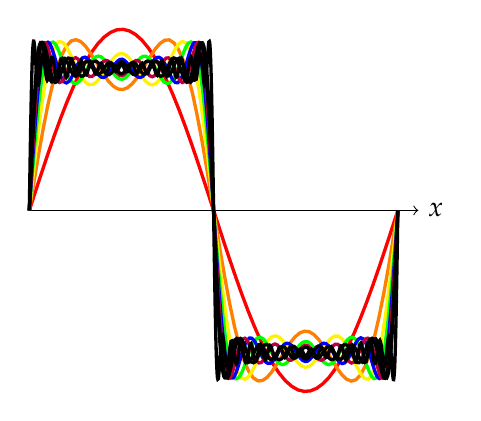
\begin{tikzpicture}[xscale=.013,yscale=2.3]
      \draw[->](0,0)--(380,0) node[pos=1,right]{$x$};
      \uncover<1>{
        \draw[samples=60,domain=0:360,red,very thick]plot({\x},{sin(\x)});
      }
      \uncover<2>{
        \draw[samples=80,domain=0:360,orange,very thick]
        plot({\x},{sin(\x)+1/3*sin(3*\x)});
      }
      \uncover<3>{
        \draw[samples=100,domain=0:360,yellow,very thick]
        plot({\x},{sin(\x)+1/3*sin(3*\x)+1/5*sin(5*\x)});
      }
      \uncover<4>{
        \draw[smooth,samples=140,domain=0:360,green,very thick]
        plot({\x},{sin(\x)+1/3*sin(3*\x)+1/5*sin(5*\x)+1/7*sin(7*\x)});
      }
      \uncover<5>{
        \draw[smooth,samples=160,domain=0:360,blue,very thick]
        plot({\x},
        {sin(\x)+1/3*sin(3*\x)+1/5*sin(5*\x)+1/7*sin(7*\x)+1/9*sin(9*\x)});
      }
      \uncover<6>{
        \draw[smooth,samples=160,domain=0:360,purple,very thick]
        plot({\x},
        {sin(\x)+1/3*sin(3*\x)+1/5*sin(5*\x)+1/7*sin(7*\x)+1/9*sin(9*\x)+
          1/11*sin(11*\x)});
      }
      \uncover<7>{
        \draw[smooth,samples=200,domain=0:360,very thick]
        plot({\x},
        {sin(\x)+1/3*sin(3*\x)+1/5*sin(5*\x)+1/7*sin(7*\x)+1/9*sin(9*\x)+
          1/11*sin(11*\x)+
          1/13*sin(13*\x)});
      }
      \uncover<8>{
        \draw[smooth,samples=200,domain=0:360,very thick]
        plot({\x},
        {sin(\x)+1/3*sin(3*\x)+1/5*sin(5*\x)+1/7*sin(7*\x)+1/9*sin(9*\x)+
          1/11*sin(11*\x)+
          1/13*sin(13*\x)+
          1/15*sin(15*\x)});
      }
      \uncover<9>{
        \draw[smooth,samples=350,domain=0:360,very thick]
        plot({\x},
        {sin(\x)+1/3*sin(3*\x)+1/5*sin(5*\x)+1/7*sin(7*\x)+1/9*sin(9*\x)+
          1/11*sin(11*\x)+ 1/13*sin(13*\x)+ 1/15*sin(15*\x)+ 1/17*sin(17*\x)+
          1/19*sin(19*\x)+
          1/21*sin(21*\x)+ 1/23*sin(23*\x)+ 1/25*sin(25*\x)+ 1/27*sin(27*\x)+
          1/29*sin(29*\x)+
          1/31*sin(31*\x)+ 1/33*sin(33*\x)+ 1/35*sin(35*\x)+ 1/17*sin(37*\x)+
          1/39*sin(39*\x)});
      }
    \end{tikzpicture}

    \column{.35\textwidth}
    \uncover<1->{
      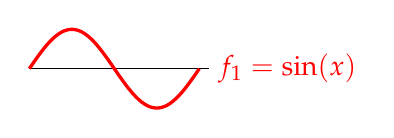
\begin{tikzpicture}[xscale=.006,yscale=.5]
        \draw(0,0)--(380,0) node[pos=1,right]{\color{red}$f_1=\sin(x)$};
        \draw[samples=60,domain=0:360,red,very thick] plot({\x},{sin(\x)});
      \end{tikzpicture}
    }
    \uncover<2->{
      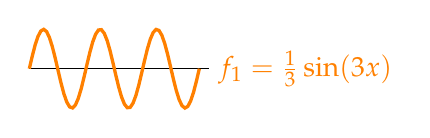
\begin{tikzpicture}[xscale=.006,yscale=.5]
        \draw(0,0)--(380,0) node[pos=1,right]
             {\color{orange}$f_1=\frac{1}{3}\sin(3x)$};
        \draw[samples=60,domain=0:360,orange,very thick] plot({\x},{sin(3*\x)});
      \end{tikzpicture}
    }
    \uncover<3->{
      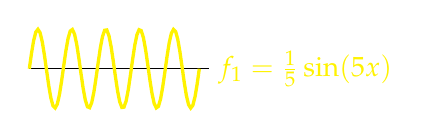
\begin{tikzpicture}[xscale=.006,yscale=.5]
        \draw(0,0)--(380,0) node[pos=1,right]
             {\color{yellow}$f_1=\frac{1}{5}\sin(5x)$};
        \draw[samples=80,domain=0:360,yellow,very thick] plot({\x},{sin(5*\x)});
      \end{tikzpicture}
    }
    \uncover<4->{
      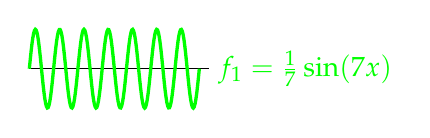
\begin{tikzpicture}[xscale=.006,yscale=.5]
        \draw(0,0)--(380,0) node[pos=1,right]
             {\color{green}$f_1=\frac{1}{7}\sin(7x)$};
        \draw[samples=200,domain=0:360,green,very thick] plot({\x},{sin(7*\x)});
      \end{tikzpicture}
    }
    \uncover<5->{
      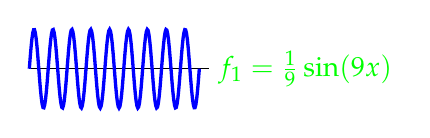
\begin{tikzpicture}[xscale=.006,yscale=.5]
        \draw(0,0)--(380,0) node[pos=1,right]
             {\color{green}$f_1=\frac{1}{9}\sin(9x)$};
        \draw[samples=200,domain=0:360,blue,very thick] plot({\x},{sin(9*\x)});
      \end{tikzpicture}
    }
  \end{columns}
\end{frame}

\begin{frame}
  \frametitle{Fourier Series and Harmonic Frequencies}

  \begin{center}
    \vspace{-.3in}
    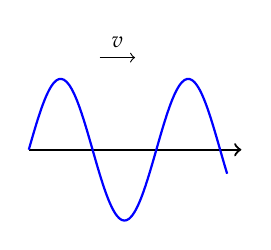
\begin{tikzpicture}[scale=.9]
      \draw[->,thick](0,0) --(3,0);
      \draw[->](1,1.3)--(1.5,1.3) node[midway,above]{\footnotesize $v$};
      \draw[thick,blue,smooth,samples=80,domain=0:2.8] plot({\x},{sin(200*\x)});
    \end{tikzpicture}
    \hspace{.15in}
    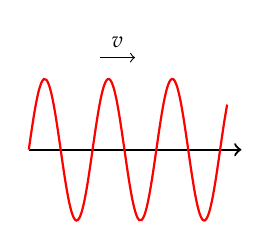
\begin{tikzpicture}[scale=.9]
      \draw[->,thick](0,0) --(3,0);
      \draw[->](1,1.3)--(1.5,1.3) node[midway,above]{\footnotesize $v$};
      \draw[thick,red,smooth,samples=80,domain=0:2.8] plot({\x},{sin(400*\x)});
    \end{tikzpicture}
    \hspace{.15in}
    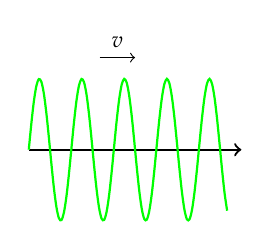
\begin{tikzpicture}[scale=.9]
      \draw[->,thick](0,0) --(3,0);
      \draw[->](1,1.3)--(1.5,1.3) node[midway,above]{\footnotesize $v$};
      \draw[thick,green,smooth,samples=80,domain=0:2.8]
      plot({\x},{sin(600*\x)});
    \end{tikzpicture}
  \end{center}

  \vspace{-.2in}
  \begin{itemize}
  \item The first wave---with the longest wavelength and lowest
    frequency---is called the \textbf{fundamental frequency}, or
    \textbf{first harmonic}
  \item The second term has half the wavelength and twice the frequency. It's
    called the \textbf{second harmonic}, the \textbf{first overtone}
  \item Also, third, fourth, fifth\ldots harmonics
  \end{itemize}
\end{frame}


\begin{frame}
  \frametitle{Harmonic Frequencies}
  \begin{itemize}
  \item When a musical instrument produces a sound, the frequency that is
    ``heard'' is the fundamental frequency
  \item Every whole-number multiples of the fundamental frequency $f_1$ is its
    harmonic frequency, i.e.\ the $n$-th harmonic is:

    \eq{-.25in}{
      \boxed{f_{\mathrm{harm},n}=nf_1}\quad\text{\normalsize where}\quad
      n\geq 1
    }
  \end{itemize}
\end{frame}

\begin{frame}
  \frametitle{Universal Wave Equation}
  When combining the wave number and angular frequency, we can find that
  the speed of a wave is the product of the wavelength and the frequency:

  \eq{-.2in}{
    \boxed{v = f\lambda}
  }
  \begin{center}
    \begin{tabular}{l|c|l}
      \rowcolor{pink}
      \textbf{Quantity} & \textbf{Symbol} & \textbf{SI Unit} \\ \hline
      Speed         & $v$       & \si{m/s} (meters per second) \\
      Frequency     & $f$       & \si{\hertz} (hertz)\\
      Wavelength    & $\lambda$ & \si{\metre} (meters) \\
    \end{tabular}
  \end{center}
  The universal wave equation applies to \emph{all} waves. For sound waves,
  $v=v_\mathrm{sound}$; for electromagnetic waves $v=c$.
\end{frame}



\begin{frame}
  \frametitle{Two Types of  Wave}
  There are two types of waves
  \begin{itemize}
  \item\textbf{Transverse waves}:
    \begin{itemize}
    \item Particles of a medium vibrate at right angles to the direction of the
      motion.
    \item e.g.: ocean waves, electromagnetic waves
    \end{itemize}
  \item\textbf{Longitudinal waves:}
    \begin{itemize}
    \item Particles of a medium vibrate parallel to the direction of the motion
      of the wave
    \item e.g.: sound waves
    \end{itemize}
  \end{itemize}
\end{frame}



\begin{frame}
  \frametitle{Transverse Wave vs.\ Longitudinal Wave}
  \begin{center}
    \pic{.6}{transverse-wave.png}\\
    \pic{.6}{compression-wave.png}
  \end{center}
\end{frame}


\begin{frame}
  \frametitle{Wave Simulation}
  A helpful simulation can be found on the PhET website at University of
  Colorado.
  \begin{center}
    \textbf{Click for external link:}\\
    \href{https://phet.colorado.edu/sims/html/wave-on-a-string/latest/wave-on-a-string_en.html}
         {wave on a string simulation}
  \end{center}
\end{frame}


\begin{frame}
  \frametitle{Wave on a String}
  The speed of a travelling wave on a stretched string is given by:

  \eq{-.2in}{
    \boxed{v=\sqrt{\frac{F_T}{\mu}}}
    \quad\text{\normalsize where}\quad
    \boxed{\mu=\frac{m}{L}}
  }
  \begin{center}
    \begin{tabular}{l|c|l}
      \rowcolor{pink}
      \textbf{Quantity} & \textbf{Symbol} & \textbf{SI Unit} \\ \hline
      Wave speed    & $v$    & \si{m/s} (meters per second) \\
      Tension       & $F_T$  & \si{\newton} (newtons)\\
      Linear mass density & $\mu$ & \si{\kilo\gram/\metre} (kilograms per meter)
      \\
      Mass of the string & $m$    & \si{\kilo\gram} (kilograms)\\
      Length of the string & $L$ & \si{\metre} (meters)
    \end{tabular}
  \end{center}
\end{frame}


\begin{frame}
  \frametitle{Power Transmitted by a Harmonic Wave}
  Then the power transmitted by a harmonic wave is through a travelling wave on
  a string is determined by the linear mass density $\mu$, the angular frequency
  $\omega$, amplitude $A$ and wave speed $v$:

  \eq{-.2in}{
    \boxed{P=\frac{1}{2}\mu\omega^2A^2v}
  }
\end{frame}


\begin{frame}
  \frametitle{The Decibel}
  The decibel is defined as by the intensity of sound $I$ compared to the
  \emph{threshold of hearing} intensity $I_0$:
  
  \eq{-.3in}{
    \boxed{\beta=10\log_{10}\left[\frac{I}{I_0}\right]}
    \;\;\text{\normalsize where}\;\; I_0=\SI{e-12}{\watt/\metre^2}
    \;\;\text{\normalsize and}\;\;
    \boxed{I=\frac{P_\mathrm{ave}}{4\pi r^2}}
  }
  \begin{center}
    \begin{tabular}{l|c|l}
      \rowcolor{pink}
      \textbf{Quantity} & \textbf{Symbol} & \textbf{SI Unit} \\ \hline
      Intensity of sound  & $\beta$ & \si{\decibel} (decibels)\\
      Intensity of sound  & $I$ & \si{W/m^2} (watts per square meters)\\
      Threshold intensity & $I_0$ & \si{W/m^2} (Watts per square meters)\\
      Average power of the source & $P_\mathrm{ave}$  & \si{\watt} (watts)\\
      Distance from the source & $r$  & \si{\metre} (meters)
    \end{tabular}
  \end{center}
  The \emph{threshold of pain} for human ears is defined at \SI{120}{\decibel}.
\end{frame}


\begin{frame}
  \frametitle{Reflection of Wave at a Boundary}
  \begin{columns}
    \column{.5\textwidth}
    When a wave on a string reflects at a boundary, how the reflected wave looks
    depends on the type of boundary
    \begin{itemize}
    \item At a \emph{fixed end} (left), the reflected wave is \emph{inverted},
      i.e.\ a crest becomes a trough
    \item At a \emph{free end} (right), the reflected wave is upright
    \end{itemize}
    
    \column{.5\textwidth}
    \pic{1}{22.jpg}
  \end{columns}
\end{frame}


\begin{frame}
  \frametitle{Transmission of Waves: Fast to Slow Medium}
  \begin{columns}
    \column{.6\textwidth}
    \begin{itemize}
    \item Reflected wave:
      \begin{itemize}
      \item Inverted, like a fixed end
      \item Same frequency and wavelength as the incoming wave
      \item The amplitude is decreased
      \end{itemize}
    \item Transmitted wave:
      \begin{itemize}
      \item Upright
      \item Same frequency as incoming wave, but has a shorter wavelength
        because the wave slowed down
      \end{itemize}
    \end{itemize}
    
    \column{.4\textwidth}
    \pic{1}{23.jpg}
  \end{columns}
\end{frame}


\begin{frame}
  \frametitle{Transmission of Waves: Slow to Fast Medium}
  \begin{columns}
    \column{.6\textwidth}
    \begin{itemize}
    \item Reflected wave:
      \begin{itemize}
      \item Upright, like a free end
      \item Same frequency and wavelength as the incoming wave
      \item The amplitude is decreased
      \end{itemize}
    \item Transmitted wave:
      \begin{itemize}
      \item Upright
      \item Same frequency as incoming wave, but has a longer wavelength because
        the wave sped up
      \end{itemize}
    \end{itemize}
    
    \column{.4\textwidth}
    \pic{1}{24.jpg}
  \end{columns}
  Note that the transmitted wave is \emph{always} upright.
\end{frame}



\section[Interference]{Wave Interference}
\begin{frame}
  \frametitle{Superposition of Waves}
  \begin{itemize}
  \item\textbf{Principle of Superposition:} When multiple waves pass through
    the same point, the resultant wave is the \emph{sum} of the waves
    \begin{itemize}
    \item A fancy way of saying that waves add together
    \end{itemize}
  \item The consequence of the principle of superposition is
    \emph{interference of waves}. There are two kinds of interference:
    \begin{itemize}
    \item\textbf{Constructive interference:} Two wave fronts (crests) passing
      through creates a wave front with greater amplitude
    \item\textbf{Destructive interference:} A crest and trough will cancel
      each other
    \end{itemize}
  \end{itemize}
\end{frame}


\begin{frame}
  \frametitle{Superposition of Waves}
  \begin{columns}
    \column{.6\textwidth}
    \textbf{Constructive interference}: In-phase wave fronts sum together
    \begin{itemize}
    \item In this example, two identical pulses move towards each other
    \item Their crests pass through A at the same time
    \item The amplitude at A when the waves pass through is higher 
    \end{itemize}
    
    \column{.4\textwidth}
    \pic{1}{constructive.png}
  \end{columns}
\end{frame}

\begin{frame}
  \frametitle{Superposition of Waves}
  \begin{columns}
    \column{.65\textwidth}
    \textbf{Destructive interference}: Out-of-phase wave fronts shows the
    difference of the wave fronts
    \begin{itemize}
    \item Two pulses move towards each other, one a crest, the other a trough
    \item They both pass through A at the same time
    \item Two waves cancel each other at A
    \end{itemize}
        
    \column{.35\textwidth}
    \pic{1}{destructive.png}
  \end{columns}
\end{frame}


\begin{frame}
  \frametitle{Standing Waves}
  If two waves of the same frequency meet up under the right conditions, they
  may appear to be ``standing still''. This is called a standing wave
  \begin{itemize}
  \item Node: A point that never moves
  \item Anti-node: A point which moves/vibrates maximally
  \end{itemize}
\end{frame}


\section[Strings]{Standing Waves on Strings}

\begin{frame}
  \frametitle{Standing Waves On a String Length $L$}
  \begin{itemize}
  \item A ``vibrating'' string is actually a standing wave on a string
  \item Both ends of the string are nodes
  \item\textbf{Resonance frequency} is a frequency that allows a standing wave
    to be created on the string. The first resonance (fundamental) frequency at
    occurs when $\lambda=2L$:
    \begin{center}
      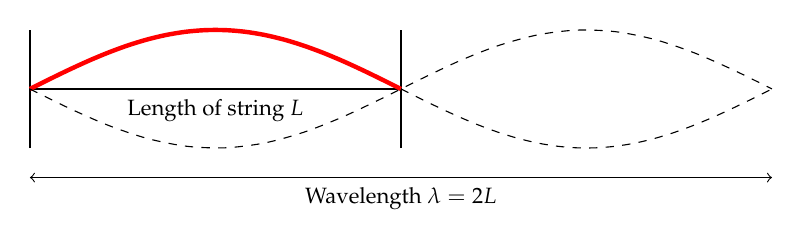
\begin{tikzpicture}[scale=1.5]
        \draw[thick](0,0) -- (pi,0)
        node[midway,below]{\footnotesize Length of string $L$};
        \draw[thick](0,-.5) --(0,.5);
        \draw[thick](pi,-.5)--(pi,.5);
        \draw[smooth,samples=20,domain=0:pi,red,ultra thick]
        plot({\x},{0.5*sin(180/pi*\x)});
        \draw[smooth,samples=20,domain=pi:2*pi,dashed]
        plot({\x},{0.5*sin(180/pi*\x)});
        \draw[smooth,samples=20,domain=0:2*pi,dashed]
        plot({\x},{-.5*sin(180/pi*\x)});
        \draw[<->](0,-.75)--(2*pi,-.75)
        node[midway,below]{\footnotesize Wavelength $\lambda=2L$};
      \end{tikzpicture}
    \end{center}
  \item Fundamental frequency is based on the speed of the
    travelling wave along the string $v_\mathrm{str}$:

    \eq{-.3in}{
      \boxed{f_1=\frac{v_\mathrm{str}}{\lambda}=\frac{v_\mathrm{str}}{2L}}
    }
  \end{itemize}
\end{frame}


\begin{frame}
  \frametitle{Standing Waves On a String Length $L$}
  A second resonance frequency happens when $L=\lambda$:

  \vspace{-.2in}
  \begin{columns}
    
    \column{.45\textwidth}
    \centering
    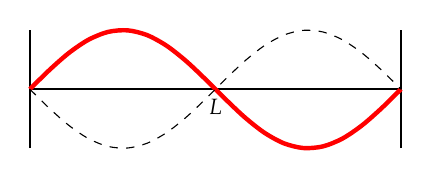
\begin{tikzpicture}[scale=1.5]
      \draw[thick](0,0)--(pi,0)  node[pos=0.5,below]{\footnotesize $L$};
      \draw[thick](0,-.5) --(0,.5);
      \draw[thick](pi,-.5)--(pi,.5);
      \draw[smooth,samples=20,domain=0:pi,red,ultra thick]
      plot({\x},{.5*sin(360/pi*\x)});
      \draw[smooth,samples=20,domain=0:pi,dashed]
      plot({\x},{-.5*sin(360/pi*\x)});
    \end{tikzpicture}
    
    \column{.55\textwidth}
    
    {\Large
      \begin{displaymath}
        f_{\mathrm{res},2}=
        \frac{v_\mathrm{str}}{\lambda}=\frac{v_\mathrm{str}}{L}=2f_1
      \end{displaymath}
    }
  \end{columns}

  \uncover<2->{
    And again, a third resonance frequency occurs at
    $\displaystyle L=\frac{3}{2}\lambda$:

    \vspace{-.2in}
    \begin{columns}
      \column{0.45\textwidth}
      \centering
      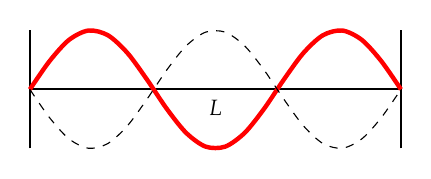
\begin{tikzpicture}[scale=1.5]
        \draw[thick](0,0) -- (pi,0)  node[pos=0.5,below]{\footnotesize $L$};
        \draw[thick](0,-.5) --(0,.5);
        \draw[thick](pi,-.5)--(pi,.5);
        \draw[smooth,samples=20,domain=0:pi,red,ultra thick]
        plot({\x},{.5*sin(540/pi*\x)});
        \draw[smooth,samples=20,domain=0:pi,dashed]
        plot({\x},{-.5*sin(540/pi*\x)});
      \end{tikzpicture}
    
      \column{.55\textwidth}
      
      {\Large
        \begin{displaymath}
          f_{\mathrm{res},3}=\frac{3v_\mathrm{str}}{2L}=3f_1
        \end{displaymath}
      }
    \end{columns}
  }
\end{frame}



\begin{frame}
  \frametitle{Standing Waves On a String Length $L$}

  In fact, the $n$-th resonance frequency of a wave on string is just:
  {\LARGE
    \begin{displaymath}
      \boxed{f_{\mathrm{res},n}=nf_1}\quad
      \text{\normalsize (standing wave on string)}
    \end{displaymath}
  }
  \begin{itemize}
  \item $f_1$ is the fundamental frequency, and $n$ is a whole-number multiple
  \item This equation is \emph{identical} to the equation for harmonic
    frequencies, meaning that every harmonic is a resonance frequency
  \item It has a ``full set of harmonics''
  \end{itemize}
\end{frame}


\begin{frame}
  \frametitle{Transfer of Sound Wave}
  Example: tuning fork
  
  \pic{.9}{tuningfork.jpg}
\end{frame}

\begin{frame}
  \frametitle{Transfer of Sound Wave}
  \framesubtitle{Schematic Diagram vs.\ Wave Graph}
  We can also express the amplitude of the sound wave by plotting the change in
  \emph{air pressure}:

  \vspace{-.2in}
  \begin{center}
    \pic{.9}{schematic-vs-graph.png}
  \end{center}
\end{frame}



\section[$v_s$]{Speed of Sound}

\begin{frame}
  \frametitle{Speed of Sound in a Gas}
  The equation for the speed of sound in a gas (e.g.\ air) is given by:

  \eq{-.2in}{
    \boxed{v_s=\sqrt{\frac{\gamma RT}{M}}}
  }
  \begin{center}
    \begin{tabular}{l|c|l}
      \rowcolor{pink}
      \textbf{Quantity} & \textbf{Symbol} & \textbf{SI Unit} \\ \hline
      Speed of sound     & $v_s$ & \si{m/s} (meters per second) \\      
      Temperature        & $T$  & \si{\kelvin} (kelvin)\\
      Universal gas constant & $R$  & \si{J/mol.K} (joule per mol per kelvin)\\
      Molar mass & $M$  & \si{\kilo\gram/mol} (kilograms per mol)\\
      Adiabatic constant  & $\gamma$  & (no units)
    \end{tabular}
  \end{center}
  For air $\gamma=1.4$, and $M=\SI{29e-3}{\kilo\gram/mol}$.
\end{frame}


%\begin{frame}
%  \frametitle{Speed of Sound in Liquids and Solids}
%  Speed of sound in a liquid depends on the ``bulk modulus'' $K$ of the liquid,
%  and density $\rho$
%      
%  \eq{-.35in}{
%    v = \sqrt{\frac{K}{\rho}}
%  }
%   
%  Speed of sound in a solid depends on the ``Young's modulus'' $E$ of the solid
%  and density $\rho$
%
%  \eq{-.35in}{
%    v = \sqrt{\frac{E}{\rho}}
%  }
%\end{frame}
%
%
%\begin{frame}
%  \frametitle{Speed of Sound in Different Media}
%  \begin{center}
%    \begin{tabular}{l|c}
%      \rowcolor{blue!30}
%      \textbf{Material} & \textbf{Speed} (\si{m/s}) \\
%      \rowcolor{pink!70}
%      \multicolumn{2}{c}{Gases (\SI{0}{\celsius}, \SI{101}{\kilo\pascal})} \\
%      Carbon dioxide & 259 \\
%      Oxygen         & 316 \\
%      Air            & 331 \\
%      Helium         & 965 \\
%      \rowcolor{pink!70}
%      \multicolumn{2}{c}{Liquids (\SI{20}{\celsius})} \\
%      Ethanol        & 1162 \\
%      Fresh water    & 1482 \\
%      Seawater (depends on depth and salinity) & 1440-1500 \\
%      \rowcolor{pink!70}
%      \multicolumn{2}{c}{Solids} \\
%      Copper         & 5010 \\
%      Glass (heat-resistant) & 5640 \\
%      Steel          & 5960
%    \end{tabular}
%  \end{center}
%\end{frame}
%
%
%\begin{frame}
%  \frametitle{Example Problem}
%  \textbf{Example 1}: Suppose the room temperature of a classroom is
%  \SI{21}{\celsius}. Calculate the speed of sound in the classroom. (Use the
%  simpler equation.)
%\end{frame}
%
%
%\begin{frame}
%  \frametitle{Example Problem}
%  \textbf{Example 2}: The temperature was \SI{4.0}{\celsius} one morning as
%  Martita hiked through a canyon. She shouted at the canyon wall, and
%  \SI{2.8}{\second} later heard an echo. How far away was the canyon wall?
%\end{frame}


\section[$M$]{Mach Number}

\begin{frame}
  \frametitle{Mach Number}
  When working with sound, it is useful to express speed in terms of its ratio
  to the speed of sound. This is called the \textbf{Mach number}:
  
  \eq{-.2in}{
    \boxed{M=\frac{v}{v_s}}
  }
  \begin{center}
    \begin{tabular}{l|c|l}
      \rowcolor{pink}
      \textbf{Quantity} & \textbf{Symbol} & \textbf{SI Unit} \\ \hline
      Mach Number         & $M$   & no units \\
      Speed of the object & $v$   & \si{m/s} (meters per second) \\
      Local speed of sound & $v_s$ & \si{m/s} (meters per second)
    \end{tabular}
  \end{center}
  \begin{itemize}
  \item When an object is travelling at $M<1$, it is travelling at a
    \emph{subsonic} speed
  \item When an object is travelling at $M>1$, it is travelling at a
    \emph{supersonic} speed
  \end{itemize}
\end{frame}



\begin{frame}
  \frametitle{Sound from a Moving Source}
  When a sound is emitted from a point source, the sound wave moves radially
  outward from the point of origin. In this diagram, the source is stationary:
  \begin{center}
    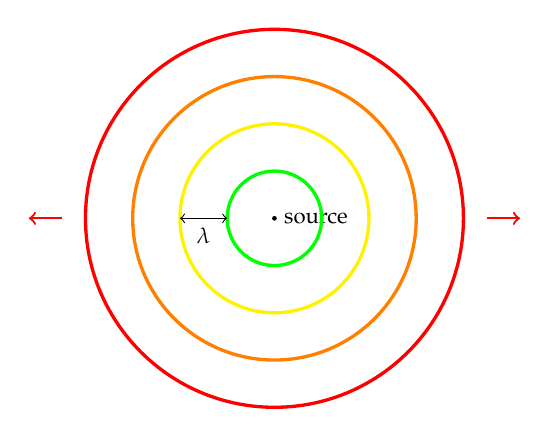
\begin{tikzpicture}[scale=.6]
      \fill[black](0,0) circle(.05) node[right]{\footnotesize source};
      \begin{scope}[very thick]
        \draw[green] (0,0) circle(1);
        \draw[yellow](0,0) circle(2);
        \draw[orange](0,0) circle(3);
        \draw[red]   (0,0) circle(4);
      \end{scope}
      \draw[<->](-1,0)--(-2,0) node[midway,below]{\footnotesize $\lambda$};
      \draw[thick,->,red](4.5,0)--(5.2,0);
      \draw[thick,->,red](-4.5,0)--(-5.2,0);
    \end{tikzpicture}
  \end{center}
\end{frame}


\section[Doppler]{Doppler Effect}

\begin{frame}
  \frametitle{Sound from a Moving Source}
  But when sound is emitted from a \emph{moving} source, the diagram looks
  different. In this case, the sound source is moving to the right, from $1$ to
  $4$:
  \vspace{.2in}
  \begin{columns}
    
    \column{.4\textwidth}
    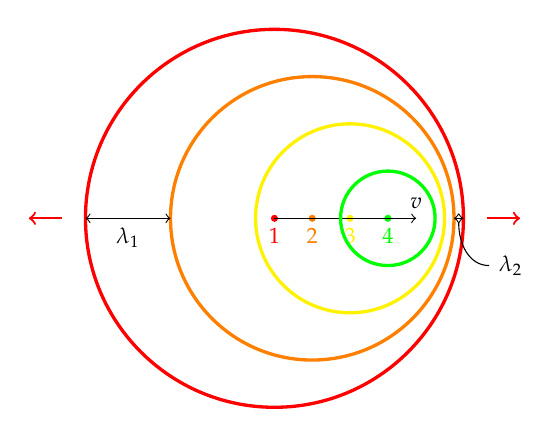
\begin{tikzpicture}[scale=.6]
      \fill[red]   ( 0,0)  circle(.075) node[below]{\footnotesize $1$};
      \fill[orange](.8,0)  circle(.075) node[below]{\footnotesize $2$};
      \fill[yellow](1.6,0) circle(.075) node[below]{\footnotesize $3$};
      \fill[green] (2.4,0) circle(.075) node[below]{\footnotesize $4$};
      \draw[->](0,0)--(3,0) node[pos=1,above]{\footnotesize $v$};
      \begin{scope}[very thick]
        \draw[red]   (  0,0) circle(4);
        \draw[orange]( .8,0) circle(3);
        \draw[yellow](1.6,0) circle(2);
        \draw[green] (2.4,0) circle(1);
      \end{scope}
      \draw[<->](-4,0)--(-2.2,0) node[midway,below]{\footnotesize $\lambda_1$};
      \draw[<->](4,0)--(3.8,0);
      \node (a) at (5,-1) {\footnotesize $\lambda_2$};
      \draw(3.9,-.1) to[out=270,in=180] (a);
      \draw[thick,->,red](4.5,0)--(5.2,0);
      \draw[thick,->,red](-4.5,0)--(-5.2,0);
    \end{tikzpicture}
      
    \column{.6\textwidth}
    \begin{itemize}
    \item When the sound source is moving \emph{towards you}, the wavelength
      $\lambda_2$ decreases, and the frequency increases.
    \item When the sound source is moving \emph{away from you}, the wavelength
      $\lambda_1$ increases, and the frequency decreases.
    \end{itemize}

    \vspace{.2in}This is called the \textbf{Doppler Effect}.
  \end{columns}
\end{frame}



%\begin{frame}
%  \frametitle{Doppler Effect}
%  We have all experienced Doppler effect before, every time an ambulance speeds
%  by us with its sirens on.
%  \begin{center}
%    \pic{.6}{toronto-ambulance.jpg}
%  \end{center}
%  When it is moving towards us, the pitch (frequency) of the siren is high,
%  but the moment it passes us, the pitch decreases!
%\end{frame}


\begin{frame}
  \frametitle{Doppler Effect}
  When a wave source is moving at a speed $v_{\textrm{src}}$ and the observer is
  moving at $v_{\textrm{ob}}$, the frequency perceived by the observer is
  shifted to $f'$:

  \eq{-.2in}{
    \boxed{f'=\frac{v_s+v_{\textrm{ob}}}{v_s-v_{\textrm{src}}}f}
  }
  \begin{center}
    \begin{tabular}{l|c|l}
      \rowcolor{pink}
      \textbf{Quantity} & \textbf{Symbol} & \textbf{SI Unit} \\ \hline
      Apparent frequency  & $f'$   & \si{hertz} (hertz) \\
      Actual frequency    & $f$    & \si{hertz} (hertz) \\
      Speed of sound      & $v_s$ & \si{m/s} (meters per second) \\
      Speed of source & $v_{\textrm{src}}$ & \si{m/s} (meters per second)\\
      Speed of observer & $v_{\textrm{ob}}$ & \si{m/s} (meters per second)
    \end{tabular}
  \end{center}
  The Doppler effect equation works for all types of waves, including sound
  waves \emph{and} electromagnetic waves.
\end{frame}


\section{Sonic Boom}

\begin{frame}
  \frametitle{Sound from a Source Moving At Sonic Speed}
  Doppler effect is more interesting is when sound source is moving at $M=1$,
  the speed of sound:
  \vspace{.2in}
  \begin{columns}
    
    \column{.4\textwidth}
    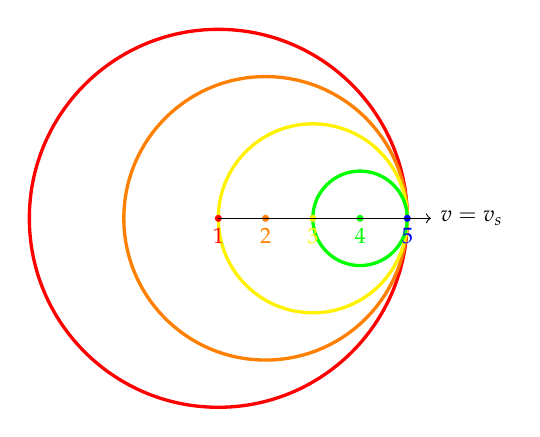
\begin{tikzpicture}[scale=.6]
      \begin{scope}[very thick]
        \draw[red]   (0,0) circle(4);
        \draw[orange](1,0) circle(3);
        \draw[yellow](2,0) circle(2);
        \draw[green] (3,0) circle(1);
      \end{scope}
      \fill[red]   (0,0) circle(.075) node[below]{\footnotesize $1$};
      \fill[orange](1,0) circle(.075) node[below]{\footnotesize $2$};
      \fill[yellow](2,0) circle(.075) node[below]{\footnotesize $3$};
      \fill[green] (3,0) circle(.075) node[below]{\footnotesize $4$};
      \fill[blue]  (4,0) circle(.075) node[below]{\footnotesize $5$};
      \draw[->](0,0)--(4.5,0) node[pos=1,right]{\footnotesize $v=v_s$};
    \end{tikzpicture}
      
    \column{.6\textwidth}
    \begin{itemize}
    \item The wave fronts (crests) from all the waves are bunched up just in
      front of the source
    \item Since sound wave is a pressure wave, right in front of the sound
      source, there is a large change in pressure (called a shock wave)
    \item When the shock passes an observer, an loud bang can be heard (aka
      \textbf{sonic boom})
    \end{itemize}
  \end{columns}
\end{frame}



\begin{frame}
  \frametitle{Sound from a Supersonic Source}
  When sound source is moving at $M>1$:
  \begin{columns}
    \column{.47\textwidth}
    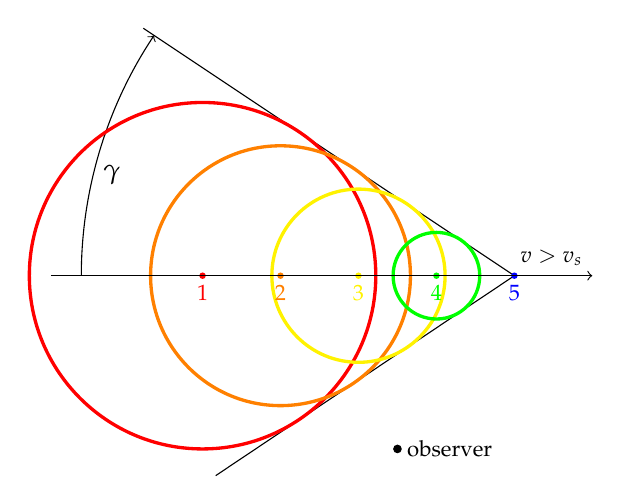
\begin{tikzpicture}[scale=.55]
      \draw[rotate around={213.8:(7.2,0)}](7.2,0)--(15.5,0);
      \draw[rotate around={146.3:(7.2,0)}](7.2,0)--(17.5,0);
      \draw[->](-2.8,0) arc(180:146.3:10) node[pos=.4,right]{$\gamma$};
      \begin{scope}[very thick]
        \draw[red]   (0,0) circle(4);
        \draw[orange](1.8,0) circle(3);
        \draw[yellow](3.6,0) circle(2);
        \draw[green] (5.4,0) circle(1);
      \end{scope}
      \fill[red]   (0,0) circle(.075) node[below]{\footnotesize $1$};
      \fill[orange](1.8,0) circle(.075) node[below]{\footnotesize $2$};
      \fill[yellow](3.6,0) circle(.075) node[below]{\footnotesize $3$};
      \fill[green] (5.4,0) circle(.075) node[below]{\footnotesize $4$};
      \fill[blue]  (7.2,0) circle(.075) node[below]{\footnotesize $5$};
      \draw[->](-3.5,0)--(9,0) node[pos=1,above left]{\footnotesize $v>v_s$};
      \fill[black](4.5,-4) circle(.1) node[right]{\footnotesize observer};
    \end{tikzpicture}
      
    \column{.53\textwidth}
    An \emph{oblique shock} is formed at an angle (called the
    \textbf{Mach angle}) given by:
      
    \eq{-.2in}{
      \gamma=\sin^{-1}\left(\frac{1}{M}\right)
    }

    A stationary observer does not hear the sound source coming until it has
    gone past!
  \end{columns}
\end{frame}


\begin{frame}
  \frametitle{Bullet in Supersonic Flight}
  Generating a shock doesn't require an actual sound source. Any object moving
  through air creates a pressure disturbance. This is a
  \SI{7.62}{\milli\metre} NATO bullet in supersonic flight.
  \begin{center}
    \pic{.35}{bullet2.jpg}
  \end{center}
  This bullet was not fired from a gun. Instead, it was placed in a shock tube
  that generates a short burst of supersonic flow, and a high-speed camera is
  then used to take the photo.
\end{frame}


\begin{frame}
  \frametitle{Duck in Water}
  No sonic booms here (just a duck swimming), but a similar shock behaviour is
  observed. The duck swims faster than the speed of the water wave, and it also
  creates a cone shape.
  \begin{center}
    \pic{.5}{duck.jpg}
  \end{center}
\end{frame}


\section{Beats}

\begin{frame}
  \frametitle{Beat Frequency}
  When waves of two different frequencies are added together, there is both
  constructive and destructive interference
  \begin{itemize}
  \item Plotting two functions representing two waves with equal magnitude
    and wave speed $v_s$: $\color{blue}{y=\sin(x)}$
    \uncover<2->{and $\color{red}{y=\sin(1.1x)}$}
  \end{itemize}
  \begin{center}
    \vspace{-.1in}
    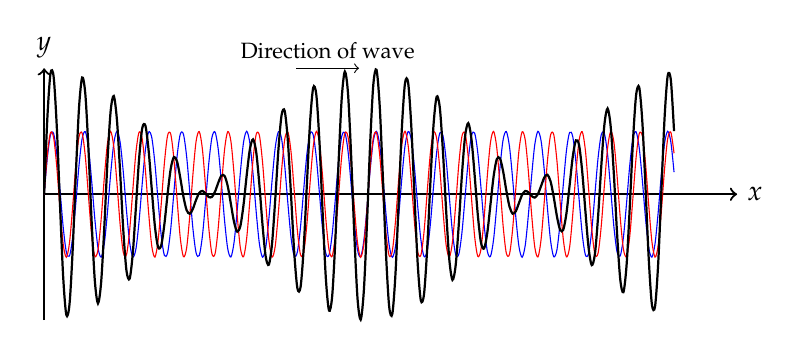
\begin{tikzpicture}[scale=.8]
      \draw[->,thick](0,0) --(11,0) node[pos=1,right] {$x$};
      \draw[->,thick](0,-2)-- (0,2) node[pos=1,above] {$y$};
      \draw[->](4,2)--(5,2) node[midway,above]{\footnotesize Direction of wave};
      \uncover<1,3->{
        \draw[blue,smooth,samples=200,domain=0:10] plot({\x},{sin(700*\x)});
      }
      \uncover<2->{
        \draw[smooth,samples=200,domain=0:10,red] plot({\x},{sin(770*\x)});
      }
      \uncover<4>{
        \draw[smooth,samples=200,domain=0:10,thick]
        plot({\x},{sin(700*\x)+sin(770*\x)});
      }
    \end{tikzpicture}
  \end{center}
  \uncover<4->{
    \vspace{-.1in}
    \begin{itemize}
    \item The thick black line is the sum: $y=\sin(x) + \sin(1.1x)$
    \end{itemize}
  }
\end{frame}



\begin{frame}
  \frametitle{Beat Frequency}
  The \emph{beat frequency} is the absolute value of the difference of the
  frequencies of the two component waves:

  \eq{-.2in}{
    \boxed{f_\mathrm{beat}=|f_1-f_2|}
  }
  \vspace{-.1in}
  \begin{center}
    \begin{tabular}{l|c|l}
      \rowcolor{pink}
      \textbf{Quantity} & \textbf{Symbol} & \textbf{SI Unit} \\ \hline
      Beat frequency     & $f_\mathrm{beat}$   & \si{\hertz} (hertz) \\
      Frequency of 1st component wave & $f_1$ & \si{\hertz} (hertz) \\
      Frequency of 2nd component wave & $f_2$ & \si{\hertz} (hertz)
    \end{tabular}
  \end{center}
\end{frame}



\section[Pipes]{Standing Waves in Pipes}

\begin{frame}
  \frametitle{Standing Waves in a Closed Pipe}
  A standing-wave patterns can be found on pipes that have both ends closed:

  \begin{center}
    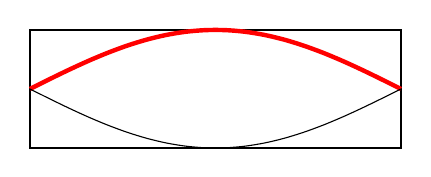
\begin{tikzpicture}[scale=1.5,yscale=.5]
      \draw[thick](0,-1) rectangle(pi,1);
      \draw[smooth,samples=20,domain=0:pi,red,ultra thick]
      plot({\x},{sin(180/pi*\x)});
      \draw[smooth,samples=20,domain=0:pi] plot({\x},{-1*sin(180/pi*\x)});
    \end{tikzpicture}
    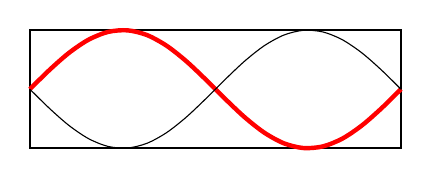
\begin{tikzpicture}[scale=1.5,yscale=.5]
      \draw[thick](0,-1) rectangle(pi,1);
      \draw[smooth,samples=20,domain=0:pi,red,ultra thick]
      plot({\x},{sin(360/pi*\x)});
      \draw[smooth,samples=20,domain=0:pi] plot({\x},{-1*sin(360/pi*\x)});
    \end{tikzpicture}\\
    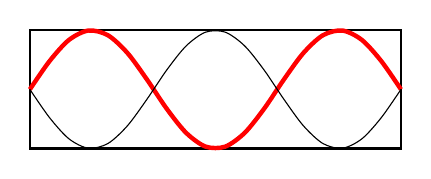
\begin{tikzpicture}[scale=1.5,yscale=.5]
      \draw[thick](0,-1) rectangle(pi,1);
      \draw[smooth,samples=20,domain=0:pi,red,ultra thick]
      plot({\x},{sin(540/pi*\x)});
      \draw[smooth,samples=20,domain=0:pi] plot({\x},{-1*sin(540/pi*\x)});
    \end{tikzpicture}
    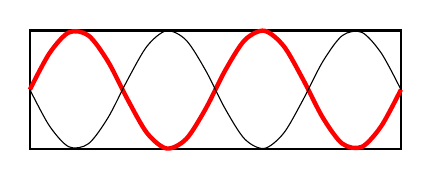
\begin{tikzpicture}[scale=1.5,yscale=.5]
      \draw[thick](0,-1) rectangle(pi,1);
      \draw[smooth,samples=20,domain=0:pi,red,ultra thick]
      plot({\x},{sin(720/pi*\x)});
      \draw[smooth,samples=20,domain=0:pi] plot({\x},{-1*sin(720/pi*\x)});
    \end{tikzpicture}
  \end{center}
\end{frame}


\begin{frame}
  \frametitle{Standing Waves in Closed Pipes}

  Like strings, pipes that are \emph{closed at both ends} also have a full set
  of harmonics. The $n$-th resonance frequency is given by:
  
  \eq{-.3in}{
    \boxed{f_{\mathrm{res},n}=nf_1}\quad\text{\normalsize (closed pipe)}
  }
  
  where $n$ is a whole-number multiple of the fundamental frequency $f_1$:

  \eq{-.25in}{
    \boxed{f_1=\frac{v_s}{2L}}
  }

  The difference between a closed pipe and a string is that the wave speed is
  now the speed of sound $v_s$ inside the pipe.
\end{frame}



\begin{frame}
  \frametitle{Standing Waves in Open Pipes}
  \begin{itemize}
  \item Example: Some organ pipes, flute
  \item Both ends of the pipes are anti-nodes
  \end{itemize}
  \begin{center}
    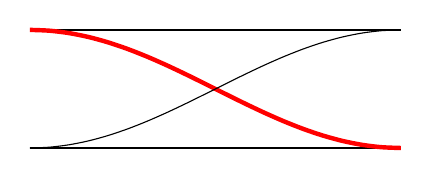
\begin{tikzpicture}[scale=1.5]
      \draw[thick](0,-.5)--(pi,-.5);
      \draw[thick](0,0.5)--(pi,0.5);
      \draw[smooth,samples=20,domain=0:pi,red,ultra thick]
         plot({\x},{0.5*sin(180/pi*\x+90)});
      \draw[smooth,samples=20,domain=0:pi]
        plot({\x},{-.5*sin(180/pi*\x+90)});
    \end{tikzpicture}
    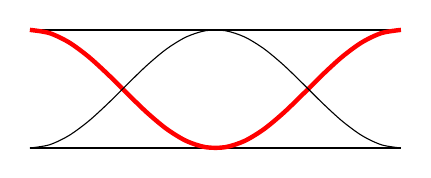
\begin{tikzpicture}[scale=1.5]
      \draw[thick](0,-.5)--(pi,-.5);
      \draw[thick](0,0.5)--(pi,0.5);
      \draw[smooth,samples=20,domain=0:pi,red,ultra thick]
        plot({\x},{0.5*sin(360/pi*\x+90)});
      \draw[smooth,samples=20,domain=0:pi]
        plot({\x},{-.5*sin(360/pi*\x+90)});
    \end{tikzpicture}\\
    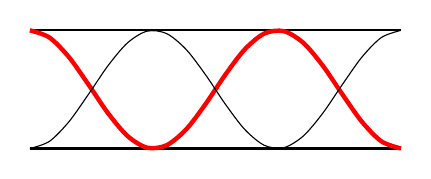
\begin{tikzpicture}[scale=1.5]
      \draw[thick](0,-.5)--(pi,-.5);
      \draw[thick](0,0.5)--(pi,0.5);
      \draw[smooth,samples=20,domain=0:pi,red,ultra thick]
      plot({\x},{0.5*sin(540/pi*\x+90)});
      \draw[smooth,samples=20,domain=0:pi]
      plot({\x},{-.5*sin(540/pi*\x+90)});
    \end{tikzpicture}
    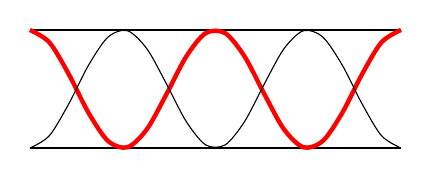
\begin{tikzpicture}[scale=1.5]
      \draw[thick](0,-.5)--(pi,-.5);
      \draw[thick](0,0.5)--(pi,0.5);
      \draw[smooth,samples=20,domain=0:pi,red,ultra thick]
      plot({\x},{0.5*sin(720/pi*\x+90)});
      \draw[smooth,samples=20,domain=0:pi]
      plot({\x},{-.5*sin(720/pi*\x+90)});
    \end{tikzpicture}
  \end{center}
  \begin{columns}
    \column{.5\textwidth}
    First resonance at $\lambda=2L$
    \begin{displaymath}
      f_1=\frac{v_s}{\lambda}=\frac{v_s}{2L}
    \end{displaymath}
    \column{.5\textwidth}
    Second resonance at $\lambda=L$
    \begin{displaymath}
      f_2=\frac{v_s}{\lambda}=\frac{v_s}{L}=2f_1
    \end{displaymath}
  \end{columns}
\end{frame}



\begin{frame}
  \frametitle{Standing Waves in Open Pipes}

  Open pipes also have a ``full set of harmonics''. The $n$-th resonance
  frequency is given by:
  
  \eq{-.3in}{
    \boxed{f_{\mathrm{res},n}=nf_1}\quad\text{\normalsize (open pipe)}
  }
  where $n$ is a whole-number multiple of fundamental frequency $f_1$:

  \eq{-.25in}{
    \boxed{f_1=\frac{v_s}{2L}}
  }
\end{frame}


\begin{frame}
  \frametitle{Standing Waves in Semi-Open Pipes}
  \framesubtitle{This is when things get a bit more interesting\ldots}
  \begin{itemize}
  \item Examples: Most organ pipes, clarinet, oboes, brass instruments
  \item Closed end: node (like in the closed pipes)
  \item Open end: anti-node (like in the open pipes)
  \end{itemize}
  \begin{center}
    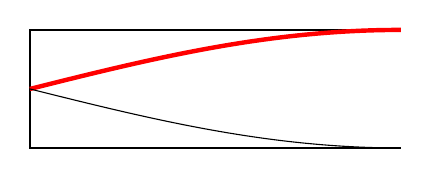
\begin{tikzpicture}[scale=1.5]
      \draw[thick](pi,-.5)--(0,-.5)--(0,.5)--(pi,.5);
      \draw[smooth,samples=20,domain=0:pi,red,ultra thick]
         plot({\x},{0.5*sin(90/pi*\x)});
      \draw[smooth,samples=20,domain=0:pi]
        plot({\x},{-.5*sin(90/pi*\x)});
    \end{tikzpicture}
    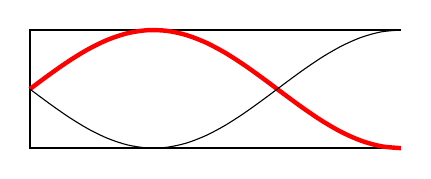
\begin{tikzpicture}[scale=1.5]
      \draw[thick](pi,-.5)--(0,-.5)--(0,.5)--(pi,.5);
      \draw[smooth,samples=20,domain=0:pi,red,ultra thick]
        plot({\x},{0.5*sin(270/pi*\x)});
      \draw[smooth,samples=20,domain=0:pi]
        plot({\x},{-.5*sin(270/pi*\x)});
    \end{tikzpicture}\\
    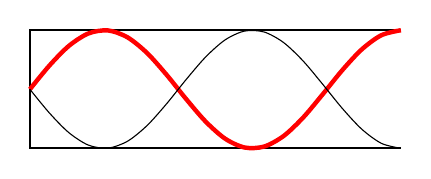
\begin{tikzpicture}[scale=1.5]
      \draw[thick](pi,-.5)--(0,-.5)--(0,.5)--(pi,.5);
      \draw[smooth,samples=20,domain=0:pi,red,ultra thick]
      plot({\x},{0.5*sin(450/pi*\x)});
      \draw[smooth,samples=20,domain=0:pi]
      plot({\x},{-.5*sin(450/pi*\x)});
    \end{tikzpicture}
    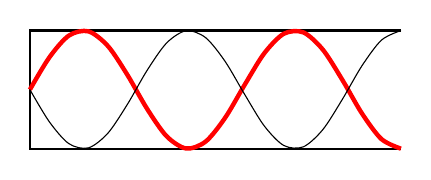
\begin{tikzpicture}[scale=1.5]
      \draw[thick](pi,-.5)--(0,-.5)--(0,.5)--(pi,.5);
      \draw[smooth,samples=20,domain=0:pi,red,ultra thick]
      plot({\x},{0.5*sin(630/pi*\x)});
      \draw[smooth,samples=20,domain=0:pi]
      plot({\x},{-.5*sin(630/pi*\x)});
    \end{tikzpicture}
  \end{center}
\end{frame}

\begin{frame}
  \frametitle{Standing Waves in Semi-Open Pipes}
  Again starting with the fundamental frequency (lowest frequency where a
  standing wave can form inside the pipe). This occurs at $\lambda=4L$:

  \vspace{-.1in}
  \begin{center}
    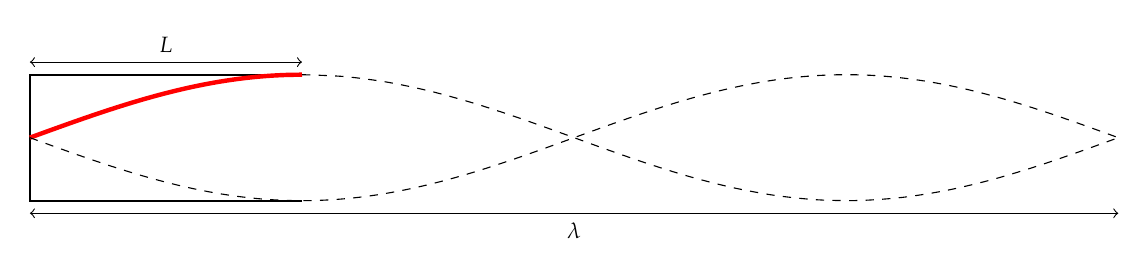
\begin{tikzpicture}[xscale=1.1,yscale=.8]
      \draw[thick](pi,-1)--(0,-1)--(0,1)--(pi,1);
      \draw[smooth,samples=20,domain=0:pi,red,ultra thick]
      plot({\x},{sin(90/pi*\x)});
      \draw[smooth,samples=20,domain=pi:4*pi,dashed]
      plot({\x},{sin(90/pi*\x)});
      \draw[smooth,samples=80,domain=0:4*pi,dashed]
      plot({\x},{-1*sin(90/pi*\x)});
      \draw[<->](0,1.2)--(pi,1.2)
      node[midway,above]{\footnotesize $L$};
      \draw[<->](0,-1.2)--(4*pi,-1.2)
      node[midway,below]{\footnotesize $\lambda$};
    \end{tikzpicture}
  \end{center}
  
  Fundamental frequency $f_1$ differs from the open-pipe and closed-pipe
  configurations by a factor of 2:

  \eq{-.2in}{
    \boxed{f_1=\frac{v_s}{\lambda}=\frac{v_s}{4L}}
  }

\end{frame}

\begin{frame}
  \frametitle{Standing Waves in Semi-Open Pipes}
  Likewise, second resonance can be found at
  $\displaystyle \lambda=\frac{4}{3}L$:
  \begin{columns}
    \column{.45\textwidth}
    \centering
    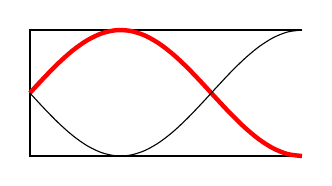
\begin{tikzpicture}[xscale=1.1,yscale=.8]
      \draw[thick](pi,-1)--(0,-1)--(0,1)--(pi,1);
      \draw[smooth,samples=20,domain=0:pi,red,ultra thick]
      plot({\x},{sin(270/pi*\x)});
      \draw[smooth,samples=20,domain=0:pi] plot({\x},{-1*sin(270/pi*\x)});
    \end{tikzpicture}
    
    \column{.55\textwidth}

    \eq{-.4in}{
      f_{\mathrm{res},2}=\frac{v_s}{\lambda}=\frac{3v_s}{4L}=3f_1
    }
  \end{columns}
  And then, third resonance at $\displaystyle \lambda=\frac{4}{5}L$:
  \begin{columns}

    \column{.45\textwidth}
    \centering
    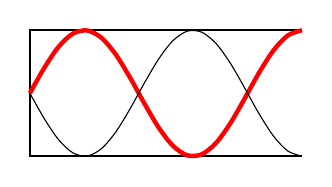
\begin{tikzpicture}[xscale=1.1,yscale=.8]
      \draw[thick](pi,-1)--(0,-1)--(0,1)--(pi,1);
      \draw[smooth,samples=20,domain=0:pi,red,ultra thick]
      plot({\x},{sin(450/pi*\x)});
      \draw[smooth,samples=20,domain=0:pi] plot({\x},{-1*sin(450/pi*\x)});
    \end{tikzpicture}

    \column{.55\textwidth}
    \eq{-.2in}{
      f_{\mathrm{res},3}=\frac{v_s}{\lambda}=\frac{5v_s}{4L}=5f_1
    }
  \end{columns}
  
  \vspace{.1in}We can repeat that for 4th, 5th\ldots resonances.
\end{frame}

\begin{frame}
  \frametitle{Standing Waves in Semi-Open Pipes}
  Only \textbf{odd-number multiples} of the fundamental frequency are resonance
  frequencies in a semi-open pipe.  We say that semi-open pipes have an
  \emph{odd} set of harmonics.

  \eq{-.25in}{
    \boxed{f_{\mathrm{res},n} = (2n-1)f_1}
    \quad\text{\normalsize (semi-open pipes)}
  }
  
  Because fundamental frequency $f_1$ is lower than open-pipe and
  closed-pipe configurations by a factor of 2 for the same length $L$, it has
  advantages when designing an organ pipe.

  \eq{-.25in}{
    \boxed{f_1=\frac{v_s}{\lambda}=\frac{v_s}{4L}}
  }
  
\end{frame}


\begin{frame}
  \frametitle{Resonance \emph{Length} in a Semi-Open Pipe}
  \begin{itemize}
  \item Now that we have looked at resonance \emph{frequencies}, we'll look
    at resonance \emph{lengths}
  \item We produce a single frequency in the pipe, and vary the length of the
    pipe until we have resonance
  \end{itemize}
\end{frame}

\begin{frame}
  \frametitle{Resonance Length in a Semi-Open Pipe}
  Let's submerge a part of this pipe in water\ldots
  \begin{center}
    \pic{.7}{res-length-closed.png}
  \end{center}
\end{frame}

\begin{frame}
  \frametitle{Resonance Length in a Semi-Open Pipe}
  The resonance lengths are \textbf{odd whole-number multiples} of the first
  resonance length $L_1$: %($\displaystyle\frac{\lambda}{4}$):
  
  \eq{-.2in}{
    \boxed{L_{\mathrm{res},n} = (2n-1)L_1}
    \quad\text{\normalsize where}\quad
    \boxed{L_1 = \frac{\lambda}{4}}
  }
\end{frame}



\begin{frame}
  \frametitle{Resonance in an Open Pipe}
  We can also repeat this with pipes that are open on both ends.
  \begin{center}
    \pic{.75}{res-length-open.png}
  \end{center}
\end{frame}



\begin{frame}
  \frametitle{Resonance in an Open Pipe}
  Resonance lengths of an open pipe are \textbf{whole-number multiples} of the
  first resonance length $L_1$:

  \eq{-.25in}{
    \boxed{L_{\mathrm{res},n}=nL_1}
    \quad\text{\normalsize (open pipe)}
  }
  
  \vspace{-.1in}where first resonance length is given by:
  
  \eq{-.2in}{
    \boxed{L_1=\frac{\lambda}{2}}
  }
  
  Be careful! This equation looks a lot like the resonance frequency equation!
\end{frame}

\end{document}
